%! Author = gacou54

% Preamble
\documentclass[11pt]{article}

% Packages
\usepackage{float}
\usepackage{amsmath}
\usepackage{hyperref}

\usepackage{tikz}
\usetikzlibrary{arrows}
\usetikzlibrary{shapes}
\usepackage{xcolor}
\usepackage{graphicx}

\usepackage[skins,listings,breakable]{tcolorbox}

% Config
\newtcblisting{code}[1][]{
  width=\linewidth,
  enhanced,
  boxrule=0.1mm,
  colback=lightgray,
  listing only,
  top=0cm,
  bottom=0cm,
  listing options={
    basicstyle=\footnotesize\ttfamily,
    language=bash,
    showstringspaces=false,
  },
  after={\par\vspace\noindent}  %% do you really need \vspace{\baselineskip}?
}

% Document information
\title{Othello User Guide}
\author{Gabriel Couture}
\setcounter{tocdepth}{2}

% Document
\begin{document}

\maketitle
\tableofcontents
\newpage

\section{Installation}\label{sec:installation}

\subsection{Install from release (preferred)}\label{subsec:install-from-release-(preferred)}
\begin{enumerate}
    \item Find the most recent release here: \url{https://github.com/ulaval-rs/othello/releases}
    \item In the assets, download the othello zip file
    \item Unzip the zip file at the path where you want the application
    \item Run \texttt{app.exe} to start the application
\end{enumerate}

\subsection{Install from source}\label{subsec:install-from-source}
Clone the repo:
\begin{code}
git clone https://github.com/ulaval-rs/othello.git
cd othello
\end{code}

\noindent Make a virtual environment:
\begin{code}
virtualenv venv
venv\Scripts\pip install -r requirements.txt
\end{code}

\noindent Re-install the \texttt{GDAL}, \texttt{Shapely}, \texttt{pyproj}, \texttt{Rtree} and \texttt{Fiona} from
\url{https://www.lfd.uci.edu/~gohlke/pythonlibs} with the following command (tested with python 3.8).
\begin{code}
venv\Scripts\pip install --force-reinstall \
  GDAL-3.2.2-cp38-cp38-win_amd64.whl
venv\Scripts\pip install --force-reinstall \
  Shapely-1.7.1-cp38-cp38-win_amd64.whl
venv\Scripts\pip install --force-reinstall \
  pyproj-3.0.1-cp38-cp38-win_amd64.whl
venv\Scripts\pip install --force-reinstall \
  Rtree-0.9.7-cp38-cp38-win_amd64.whl
venv\Scripts\pip install --force-reinstall \
  Fiona-1.8.18-cp38-cp38-win_amd64.whl
\end{code}

\subsubsection{Setup the ESRI geodatabase (.gdb) driver support}
\noindent You need 2 files for this: \texttt{ogr\_FileGDB.dll} and \texttt{FileGDBAPI.dll}.
gohlke's GDAL library comes with the \texttt{ogr\_FileGDB} driver as a plugin.
\texttt{ogr\_FileGDB.dll} is found at \texttt{venv\Lib\site-packages\osgeo\gdalplugins\disable\ogr\_FileGDB.dll}.
Simply copy and paste the file outside the disable directory: \texttt{venv\Lib\site-packages\osgeo\gdalplugins\ogr\_FileGDB.dll}. \\


\noindent The \texttt{FileGDBAPI.dll} is the proprietary SDK from ESRI .
It can be found on the following repository: \url{https://github.com/Esri/file-geodatabase-api/blob/master/FileGDB_API_1.5.1/FileGDB_API_1_5_1-VS2017.zip}.
Unpack the zip file and copy-paste the \texttt{bin64\FileGDPAPI.dll} to \texttt{venv\Lib\site-packages\osgeo\FileGDPAPI.dll}.
The ESRI geodatabase driver support should then be enabled.

\subsubsection{Build Othello}
\noindent Build the application to the \texttt{build} directory with the following command.
\begin{code}
venv\Scripts\python3.8 setup.py build
\end{code}


\newpage
\section{Usage}\label{sec:usage}
Othello is a tool that allows you to link optimization data from Macbeth software
and geographic data in GDB format (ArcGIS proprietary format).
It consists of two tools: the first being \textit{Criteria}, and the second \textit{Aggregate}.

\subsection{\textit{Criteria}}\label{subsec:criteria}
The \textit{Criteria} allows to transform the values of a criterion thanks
to a scale present in a macbeth file.
The data flow is schematized in the \ref{fig:criteria-tool} image.
Essentially, a column from an ArcGIS GDB file is combined
with a linear relation extracted from a MacBeth file to produce
a new column in the ArcGIS GDB file.
The linear relation from the MacBeth file is in fact an interpolation from two columns.

\begin{figure}[H]
    \centering
    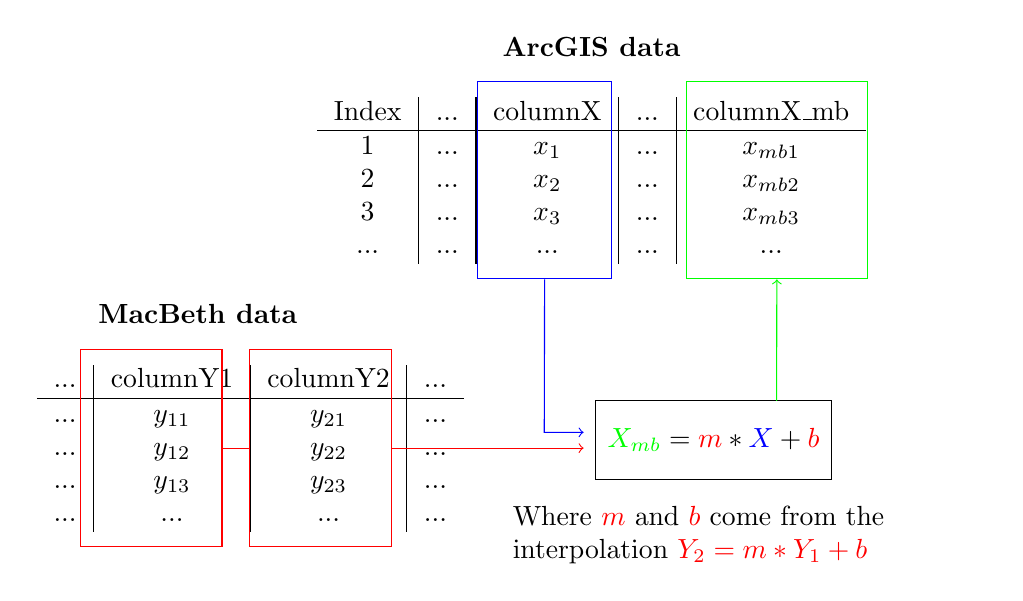
\begin{tikzpicture}
    % Tables
    \node (tab1) {%
        \begin{tabular}{c|c|c|c|c}
            Index  & ... & columnX & ... & columnX\_mb \\
            \hline
            1 & ... & $x_1$ & ... & $x_{mb1}$ \\
            2 & ... & $x_2$ & ... & $x_{mb2}$ \\
            3 & ... & $x_3$ & ... & $x_{mb3}$ \\
            ... & ... & ... & ... & ...
        \end{tabular}
    };
    \node [left,xshift=-1.5cm,yshift=-3.4cm] (tab2) {%
        \begin{tabular}{c|c|c|c}
            ... & columnY1 & columnY2 & ...\\
            \hline
            ... & $y_{11}$ & $y_{21}$ & ...\\
            ... & $y_{12}$ & $y_{22}$ & ...\\
            ... & $y_{13}$ & $y_{23}$ & ... \\
            ... & ... & ... & ...
        \end{tabular}
    };

    % Table labels
    \node[yshift=1.7cm] {\textbf{ArcGIS data}};
    \node[xshift=-5cm, yshift=-1.7cm] {\textbf{MacBeth data}};

    % Rectangles
    \node [
        rectangle,
        draw=blue,
        right,
        xshift=-1.45cm,
        minimum width=1.7cm,
        minimum height=2.5cm,
    ] (rec-x) {};
    \node [
        rectangle,
        draw=red,
        right,
        xshift=-6.5cm,
        yshift=-3.4cm,
        minimum width=1.8cm,
        minimum height=2.5cm,
    ] (rec-y1) {};
    \node [
        rectangle,
        draw=red,
        right,
        xshift=-4.35cm,
        yshift=-3.4cm,
        minimum width=1.8cm,
        minimum height=2.5cm,
    ] (rec-y2) {};
    \node [
        rectangle,
        draw=green,
        right,
        xshift=1.2cm,
        minimum width=2.3cm,
        minimum height=2.5cm,
    ] (rec-mb) {};
    \node [
        draw,
        rectangle,
        xshift=1.55cm,
        yshift=-3.3cm,
        minimum width=3cm,
        minimum height=1cm,
    ] (rec) {
        $\textcolor{green}{X_{mb}} = \textcolor{red}{m} * \textcolor{blue}{X} + \textcolor{red}{b}$
    };

    % Labels
    \node [xshift=2cm, yshift=-4.5cm, text width=6cm] {
        Where $\textcolor{red}{m}$ and $\textcolor{red}{b}$ come from the\\
        interpolation $\color{red} Y_2 = m * Y_1 + b$
    };

    % Arrows
    \draw [->, blue] (rec-x) -- (-0.6cm,-3.2cm) -- (-0.1cm,-3.2cm);
    \draw [-, red] (rec-y1) -- (rec-y2);
    \draw [->, red] (rec-y2) -- (-0.1cm,-3.4cm);
    \draw [->, green] (2.35cm,-2.8cm) -- (rec-mb);

\end{tikzpicture}
    \caption{Criteria tool data flow diagram}
    \label{fig:criteria-tool}
\end{figure}

Figure~\ref{fig:criteria-ui} shows the user interface where you can use this tool.
From this tool, it is possible to load an ArcGIS GDB file,
to choose the right layer and finally the column which will be the source one
(columnX in blue in the figure~\ref{fig:criteria-tool}).

\begin{figure}[H]
    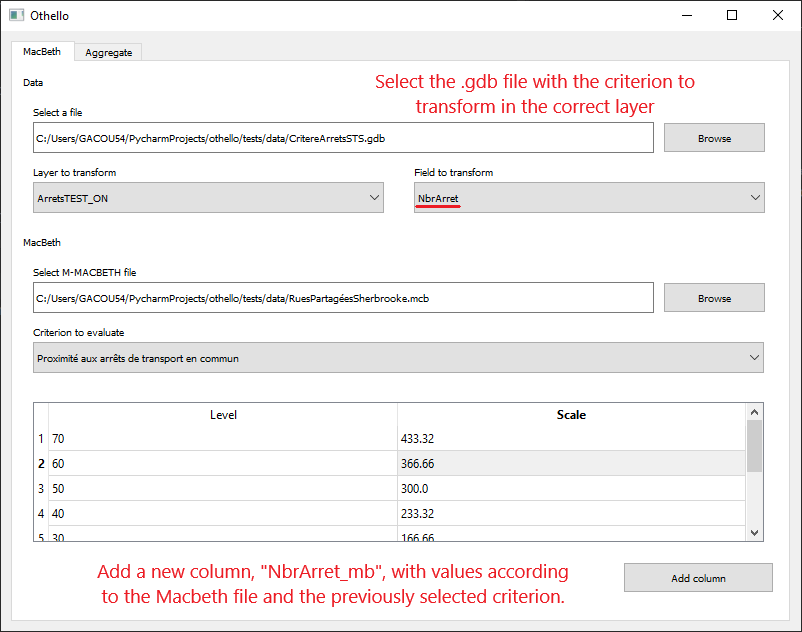
\includegraphics[width=\linewidth]{../images/criteria_tool.png}
    \caption{\textit{Criteria} tool's user interface}
    \label{fig:criteria-ui}
\end{figure}

\subsection{\textit{Aggregate}}\label{subsec:aggregate}

\end{document}
